\documentclass[a4paper,10pt]{article}
\usepackage[utf8]{inputenc}
\usepackage{amsfonts,amsmath,amssymb,amsthm,amstext,latexsym}	
\usepackage{tikz}
\usetikzlibrary{calc}
\usetikzlibrary{arrows,shapes}
\usetikzlibrary{patterns,snakes}
%opening
\title{Approximating a Multi-Grid Solver}
\author{Valentin Le Fèvre}

\begin{document}

\maketitle

\section{Introduction}

The multi-grid algorithms are a class of linear system solvers.
The idea is to restrict and interpolate vectors and matrices to have easier problems to solve, that is, problems that we can solve in much less time than the original one.

We will focus on a quite general and simple multi-grid solver implemented using the HYPRE library.

\section{Definitions}

\begin{itemize}
 \item A system of equations is represented by the following equation: $Ax=b$, where $A \in \mathcal{M}(\mathbb{R})^{n\times n}$ and $b \in \mathcal{\mathbb{R}}^n$ are given and
 $x \in \mathbb{R}^n$ is the unknown. The \emph{exact} solution of this system will be denoted by $\widetilde{x}$.
 \item A level is an integer between $1$ and $L$. Level $1$ will be called the finest level, and level $L$ will be called the coarsest level.
 \item The restriction of $A$ (or $b$ or $x$) to level $l$ will be denoted by $A^l$ (or $b^l$ or $x^l$). We have $A^1 = A$ (and $b^1=b,x^1=x$).
 \item We define a set of $L-1$ restriction matrices $R_1,\dots,R_{L-1}$ such that $R_l b^l = b^{l+1}$. We also define some prolongation matrices $P_1,\dots,P_{L-1}$ such that $P_{l}b^{l+1} = b^l$.
 In other words, we have $P_l = {R_l}^T$ and we build the $A^l$ matrices as follows: $A^{l+1} = R_l A^l P_l$.
 \item We denote by $e^l$ the error at level $l$, that is the vector such that $x^l + e^l = \widetilde{x^l}$, that is to say $\widetilde{x^l}-x^l$.
 We also define the residual at level $l$, $r^l = b^l - A^lx^l$. As $b^l = A^l\widetilde{x^l}$, we can also write $r^l = A^le^l$.
 \item We derive the relative residual norm at any step $i$ in the algorithm
 by the norm of the residual at this step, $||b^l - A^lx^l_i||$, divided by the norm of the initial residual, $|| b^l - A^lx^l_0||$.\\ We also define the notion of \emph{tolerance}
 as an real value between 0 and 1, which is a threshold for stopping an algorithm. In multi-grid algorithms, this threshold will be on the residual norm.
 \item We call relaxation a step of an iterative method for solving linear systems (such as Jacobi, Gauss-Sneidel, \dots). Formally, for a vector $x \in \mathbb{R}^n$, it represents the computation of
 $x \leftarrow Mx + c$ where $M \in \mathcal{M}(\mathbb{R})^{n\times n}$ and $c \in \mathcal{\mathbb{R}}^n$ and are defined depending on the method used.
\end{itemize}

\section{How it works}

  The goal of the algorithm is to improve the efficiency of iterative methods. Indeed, the choice of the starting vector $x$ on which to apply relaxations has consequences on the convergence
  time of the solver, and depending on the system to solve, the convergence of factor (related to the matrix $M$) can be close to 1.\\
  Here the idea is to do some relaxations and then correct the value of $x$ by adding it the corresponding error term. However, this error term cannot be computed easily (otherwise,
  solving the problem would be done by computing the error term and adding it to $x$). Multi-grid solvers instead use recursion to compute the error term. The stopping parameter for the
  recursion will be determined by decreasing the sizes of vectors and matrices (thus loosing on precision but saving time).
  Formally, we can sum up the algorithm as follows:
  
  MG$(l,x,f,\alpha_1,\alpha_2)$:
  \begin{itemize}
    \item If $l = L$, return $x = {A^L}^{-1} f$ (exact solve);
    \item Else:
    \begin{enumerate}
      \item Relax $x$ $\alpha_1$ times using an iterative method (matrix $A^l$, right hand side $f$);
      \item $r \leftarrow R_l ( f - Ax )$;
      \item $y \leftarrow 0$:
      \item MG$(l+1,y,r,\alpha_1,\alpha_2)$;
      \item $e \leftarrow P_{l} y$;
      \item $x \leftarrow x+e$;
      \item Relax $x$ $\alpha_2$ times using an iterative method (matrix $A^l$, right hand side $f$);
   \end{enumerate}
  \end{itemize}
  The algorihtm is then executed by setting $x^l \leftarrow 0$ and then executing MG$(1,x^l,b^l,\alpha_1,\alpha_2)$.

  Then several ways of modifying the algorithm appear:
  \begin{itemize}
   \item Which iterative method to use?
   \item Do we want only one recursion or more?
   \item How many times do we need to apply the algorithm?
   \item How to determine good $\alpha_1$ and $\alpha_2$ parameters?
   \item How many levels should be defined?
  \end{itemize}

  In all what follows the iterative method chosen is an hybrid Jacobi/Gauss-Seidel method. The number of levels used will not be studied.
  
\section{Comparison of existing strategies}

  In this section, we will compare different types of cycles and study how the number of relaxation steps influence the convergence of the algorithm.
  
  We will consider 2 types of cycles: the V-cycle and the W-cycle. The V-cycle is actually the algorithm previously described. The W-cycle looks the same but instead of having two parameters
  $\alpha_1$ and $\alpha_2$ we add a new $\alpha_3$ parameter. It will represent the number of relaxation steps done after a second recursive call. In terms of algorithm it is the same
  algorithm as the V-cycle but the bullets 2 to 7 are repeated. We call these cycles V-cycle and W-cycle because of how we can draw this is we represent each time relaxations are done
  at a level by a point (see Figure~\ref{fig.cycles}). It is possible to define other types of cycles by adding more and more repeats of these steps (repeat $k$ times those steps) to generalize
  the notion of cycle to a $k$-cycle (where a V-cycle is a $1$-cycle and a W-cycle is a $2$-cycle).
  
 \begin{figure}
 %\resizebox{\linewidth}{4cm}{
 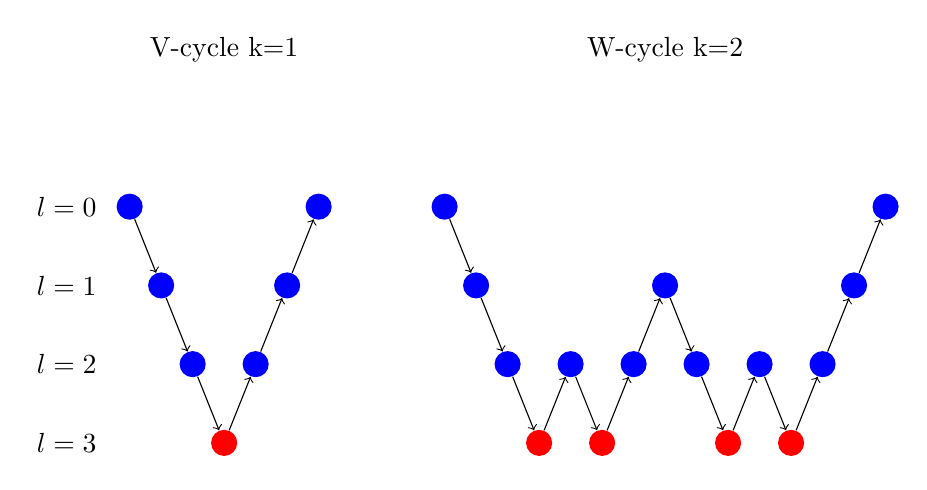
\begin{tikzpicture}
 
 
\begin{scope}[xscale=2/5]

  \node (sh) at (-5,3) { $l=0$ };
  \node (shh) at (-5,2) { $l=1$ };
  \node (shhh) at (-5,1) { $l=2$ };
  \node (shhhh) at (-5,0) { $l=3$};
  
  \node (title) at (0,5) { V-cycle k=1};
  \node (title2) at (14,5) {W-cycle k=2};

    \node[circle,fill=blue] (a) at (-3,3) { };
    \node[circle,fill=blue] (b) at (-2,2) {};
    \node[circle,fill=blue] (c) at (-1,1) {};
    \node[circle,fill=red] (d) at (0,0) {};
    \node[circle,fill=blue] (e) at (1,1) {};
    \node[circle,fill=blue] (f) at (2,2) {};
    \node[circle,fill=blue] (g) at (3,3) {};
    
    \draw[->] (a) -- (b);
    \draw[->] (b) -- (c);
    \draw[->] (c) -- (d);
    \draw[->] (d) -- (e);
    \draw[->] (e) -- (f);
    \draw[->] (f) -- (g);
    
    \node[circle,fill=blue] (aa) at (7,3) { };
    \node[circle,fill=blue] (ab) at (8,2) {};
    \node[circle,fill=blue] (ac) at (9,1) {};
    \node[circle,fill=red] (ad) at (10,0) {};
    \node[circle,fill=blue] (ae) at (11,1) {};
    \node[circle,fill=red] (af) at (12,0) {};
    \node[circle,fill=blue] (ag) at (13,1) {};
    \node[circle,fill=blue] (ah) at (14,2) {};
    \node[circle,fill=blue] (ai) at (15,1) {};
    \node[circle,fill=red] (aj) at (16,0) {};
    \node[circle,fill=blue] (ak) at (17,1) {};
    \node[circle,fill=red] (al) at (18,0) {};
    \node[circle,fill=blue] (am) at (19,1) {};
    \node[circle,fill=blue] (an) at (20,2) {};
    \node[circle,fill=blue] (ao) at (21,3) {};
    
    \draw[->] (aa) -- (ab);
    \draw[->] (ab) -- (ac);
    \draw[->] (ac) -- (ad);
    \draw[->] (ad) -- (ae);
    \draw[->] (ae) -- (af);
    \draw[->] (af) -- (ag);
    \draw[->] (ag) -- (ah);
    \draw[->] (ah) -- (ai);
    \draw[->] (ai) -- (aj);
    \draw[->] (aj) -- (ak);
    \draw[->] (ak) -- (al);
    \draw[->] (al) -- (am);
    \draw[->] (am) -- (an);
    \draw[->] (an) -- (ao);
    \end{scope}
    
 \end{tikzpicture}
 \caption{V-cycle and W-cycle on 4-level grid.}
 \label{fig.cycles}
\end{figure}

A strategy will be composed of a type of cycle (V or W) and a number of relaxation steps $\alpha$. The default implementation of BomerAMG does not allow to have different for values
for $\alpha_1,\alpha_2,\dots$ so we set them all to this value $\alpha$. We consider a total of 8 different stragies represented in Table~\ref{table.strat1}.
To compare the different strategies using the BoomerAMG algorithm, we run the algorithm on a predefined matrix of size $512000 \times 512000$ for every
value of maximum number of iterations (i.e. number of cycles) from 1 to 100 and with a required tolerance of $0$ (meaning
that the algorithm will stop when the result is exact or the maximum number of iterations is reached). We measure for each experiment the final relative residual norm and the execution time. Each experiment is run 10 times to have an accurate average execution time.
The results are presented on Figures~\ref{fig.first_tests} and \ref{fig.first_tests_time}.

\begin{table}

\begin{center}
 \begin{tabular}{|c|c|c|c|c|c|c|c|c|}
   \hline
   Type of cycle & V & V & V & V & W & W & W & W \\
   \hline
   $\alpha$ & 1 & 2 & 3 & 10 & 1 & 2 & 3 & 10 \\
   \hline
 \end{tabular}
\end{center}
 \caption{8 strategies.}
 \label{table.strat1}

\end{table}


\begin{figure}
  \includegraphics[width=\linewidth]{figs/convergence_1.pdf}
  \caption{Execution time and final residual norm as a function of the maximum number of iterations.}
  \label{fig.first_tests}
\end{figure} 

\begin{figure}
  \includegraphics[width=\linewidth]{figs/time_convergence.pdf}
  \caption{Execution time as a function of the final residual norm.}
  \label{fig.first_tests_time}
\end{figure}

\end{document}
